\section{The Statistical Interpretation of Quantum Mechanics\cite{Breuer2002}}
Consider a statistical ensemble $\varepsilon$ consisting of a suitably large number N of identically prepared quantum systems
\begin{equation}
  \varepsilon = \{S^1, S^2, \ldots, S^N\}
\end{equation}
Such a statistical ensemble represents a particular set of experimental conditions, whose realisation in each instance generates a particular member $S^i$ of  $\varepsilon$

The first postulate of the statistical interpretation of quantum mechanics is that a complete characterisation of such a statistical ensemble can be represented by a normalised state vector $| \psi \rangle$ in an associated Hilbert space $\mathcal{H}$

The second postulate is that all the possible outcomes of measurements on such an ensemble are represented by self-adjoint operators on $\mathcal{H}$.
The outcome of the measurement corresponding to an operator $\hat{R}$ represents a real valued random variable R with cumulative distribution function $F_{\hat{R}}$ defined via the family of orthogonal projection operators that constitute the spectral decomposition of $\hat{R}$:
\begin{equation}
  \hat{R} = \int_{-\infty}^\infty rdE_r
\end{equation}
as
\begin{equation}
  F_{\hat{R}} = \langle \psi |E_r | \psi \rangle
\end{equation}
This characterisation of the possible statistical variation of a quantum system is not yet complete, for it neglects classical uncertainty associated with which statistical ensemble $\varepsilon$ represents a given quantum system.
To generate the most general possible representation of a quantum statistical ensemble, a number of possible quantum ensembles $\varepsilon_\alpha$ of the above type are mixed with weights $w_\alpha$ (these weights are probabilities in the classical, not quantum sense).
A self-adjoint operator now yields a random variable R with cumulative distribution function
\begin{equation}
  F_{\hat{R}} = \sum_\alpha w_\alpha \langle \psi_\alpha | E_r | \psi_\alpha \rangle
\end{equation}
for convenience, the \emph{density operator} $\rho$ can be introduced thus
\begin{equation}
  \dens = \sum_\alpha w_\alpha |\psi_\alpha \rangle \langle \psi_\alpha |
\end{equation}
and the cumulative distribution written:
\begin{equation}
  F_{\hat{R}} = tr\{E_r \dens \}
\end{equation}
by a similar mixing argument and using the spectral decomposition of $\hat{R}$ the mean and variance of the random variable associated with $\hat{R}$ as above are as follows
\begin{align}
  \langle \hat{R} \rangle &= tr\{\hat{R} \dens \} \\
  var(\hat{R}) &= \langle \hat{R}^2 \rangle - {\langle \hat{R} \rangle}^2
\end{align}
The density matrix constitutes a complete description of the statistical properties of an open quantum system.
Thus, the dynamics of such a system can be described by the time evolution of its density operator.
\section{The Quantum Master Equation}
The quantum master equation is a generalisation of the classical master equation, which describes the time evolution of a system confined to a set of states, to the case where quantum correlations between different states are important. 

In the nonrelativistic theory of quantum mechanics the time evolution of the pure state state vector is described by the \emph{Schr\"odinger equation}:
\begin{equation}
	i\hbar \frac{d}{dt} |\psi(t)\rangle = \ham(t) |\psi(t) \rangle
        \label{eq:schrodingerequation}
\end{equation}
with $\ham$ the Hamiltonian of the system.
Setting $\hbar$ to 1 going forwards, the time dependence in the above can also be represented in terms of a time evolution operator (generated by the Hamiltonian)
\begin{equation}
        |\psi(t) \rangle = U(t, 0) | \psi(0) \rangle 
        \label{eq:timeevolutionoperator}
\end{equation}
by substitution of \cref{eq:timeevolutionoperator} into \ref{eq:schrodingerequation}, it is easy to see that $U^{\dagger}U = UU^\dagger = I$ provided $\ham$ is hermitian i.e. U represents unitary time evolution of the system

For a mixed state of a closed system, an equation of motion for the density matrix
\begin{equation}
	\dens (t) = \sum_\alpha w_{\alpha} |\psi_\alpha (t) \rangle \langle \psi_\alpha (t) |
\end{equation}
can be found by propagating each normalised $| \psi_\alpha (t) \rangle$ with the time evolution operator, the result of which is more concisely expressed
\begin{equation}
	\dens (t) = U(t, 0)\dens (0) U^\dagger (t, 0)
\end{equation}
which, when differentiated with respect to time yields the \emph{Liouville-Von Neumann} equation
\begin{equation}
	\frac{d}{dt}\dens(t) = i [\ham, \dens (t) ]
\end{equation}
For open quantum systems, i.e. those coupled to other systems, the dynamics are in general not unitary. 
Mathematically, we partition a larger, unitarily evolved system into system and environment, and perform a partial trace over the environment degrees of freedom.

We start with the Hamiltonian for a closed, potentially mixed, potentially time dependent quantum system and partition it into components representing: a subsystem constituting the totality of the interesting dynamics: the \emph{system}, a subsystem representing the dynamics of the remaining subsystem the \emph{environment} or \emph{reservoir}, and a component representing the interaction between system and environment (there is an associated partitioning of the Hilbert space into the tensor product of system and environment Hilbert spaces, and in the equation below it is understood that operators with the subscript S operate only on the system degrees of freedom i.e. exist in the system Hilbert space and represent identity in the environment Hilbert space, and etc.)
\begin{equation}
	\ham = \ham_S +\ham_R + \ham_I
\end{equation}
The partial trace operation is an operator-valued function that takes a operator on a larger Hilbert space and discards its action on all but a smaller Hilbert space, colloquially ``tracing over'' the degrees of freedom of the discarded subsystem to leave the operator on a smaller subsystem.

Unitarily evolving the large system, and performing the partial trace
\begin{equation}
	\dens_S (t) = tr_E \{U(t, 0) \dens (0) U^\dagger (t, 0) \}
\end{equation}
with $\dens_S = tr_E\{\dens \}$ we arrive at the most general form for evolution of a subsystem, also known as the reduced master equation
\begin{equation}
	\frac{d}{dt} \rho_S (t) = -itr_E\{[\ham(t), \dens_S(t)]\}
\end{equation}
Which is presented here in full generality. We now consider solvable approximations, and alternative conceptualisations.
\subsection{Quantum Measurements}
One general theory of non unitary evolution is furnished by the generalised theory of quantum measurement \cite{Wiseman2010a}
\subsubsection{Von-Neumann projective measurements}
The standard formulations of quantum mechanics considers measurements via the Von-Neumann-L\"uders Projection Postulate\cite{Dirac1927}
\newtheorem{definition}{Definition}
\begin{definition}
    The result of a measurement of operator $A$ with spectral decomposition $A = \sum_\lambda \lambda \hat{\Pi}_\lambda $, (for $A$ with discrete, non-degenerate spectrum) is an eigenvalue $lambda$, and state of the system conditioned on receiving such a value is given by
    \begin{equation}
        \rho_\lambda = \frac{\hat{\Pi}_\lambda \rho \hat{\Pi}_\lambda}{Tr[\rho\hat{\Pi}_\lambda]}
    \end{equation}
\end{definition}
The quantum analog of the Bayesian rule for the update of probabilities.
In general, such a description does not represent the measurements that experimentalists perform on quantum systems, and nor does it consider the coupling of every real quantum system to its environment.
More generally, we deal with the formalism of Operators \& Effects.
We consider a probe (or pointer/meter/apparatus) system through which we measure the system of interest.
Let the initial state of the combined probe-system state be a pure product of probe-system kets
\begin{equation}
  | \Psi (t) \rangle = | \theta (t) \rangle \otimes | \psi (t) \rangle
\end{equation}
We let the coupled system evolve unitarily for some time $t_1$, entangling the system and the probe.
We now perform a Von-Neumann projective measurement on the probe, through some projector $\pi_\lambda = \Pi_\lambda \otimes \hat{I}$ acting only on the probe space over some second period of time $t_2$ with $t_1 + t_2 = T$.
From the projection postulate, we have as conditional final state:
\begin{equation}
    | \Psi_\lambda (t+T) \rangle = \frac{\pi_\lambda U(t_1) |\Psi(t)\rangle}{P}
\end{equation}
where P is the probability that we obtain result $\lambda$ when measuring the probe.
Measuring the entangled state projectively disentangles the probe and the system and represents an operation on the system space given by
\begin{equation}
\Psi_\lambda = | \lambda \rangle \hat{M}_\lambda | \psi(t) \rangle / P
\end{equation}
where we implicitly consider nondegenerate spectra by decomposing the projector $\Pi_\lambda = |\lambda \rangle \langle \lambda |$, and where
\begin{equation}
     \hat{M}_\lambda = \langle \lambda | U(t_1) | \theta(t) \rangle
\end{equation}
is the \emph{measurement operator}, which now acts only only on the system Hilbert space.
The normalisation factor P is expressed in terms of these operators
\begin{equation}
     P^2 = \langle \Psi (t) | \hat{M}_\lambda^\dagger \hat{M}_\lambda | \Psi (t) \rangle
\end{equation}
 Our description of the measurement process has been so far effectively independendent of the meter.
We can thus abstract over the particular form of the probe state.
The state of the system following the generalised measurement process is given through the measurement operators $\hat{M}_\lambda$ as follows
\begin{equation}
 | \psi_\lambda (t + T) \rangle = \hat{M}_\lambda | \psi(t) \rangle /P
\end{equation}
 and the probability that the system takes some state is given through the \emph{effects} (probability operators) $ \mathscr{E}_\lambda = \hat{M}_\lambda^\dagger \hat{M}_\lambda $ as
\begin{equation}
     P^2 = \mathscr{P}_\lambda = \langle \psi_\lambda (t) | \mathscr{E}_\lambda | \psi_\lambda \rangle
\end{equation}
 the set $\{\mathscr{E}_\lambda | \sum_\lambda \mathscr{E}_\lambda = \hat{I} \} $ is known as a POVM: a \emph{Positive Operator Valued Measure} \footnote{Positivity is clear since the operators $\hat{M}_\lambda$ are positive.
Positivity, and that the operators resolve unity constitute the only restrictions on these operators}
We now consider a finite sequence of quantum measurements of this kind.
From the above, after some given timestep T, (we now consider propagating mixed states rather than pure states)
\begin{equation}
     \rho_\lambda (T) = \mathscr{F}_T[\hat{M}_\lambda] \rho(0) / \mathscr{P}_\lambda
\end{equation}
With $\mathscr{F}_T[\hat{M}_\lambda] ( \hat{O} ) =  \hat{M}_\lambda \hat{O} \hat{M}_\lambda ^ \dagger$ a \emph{superoperator}
This superoperator is an \emph{operation} for the value $\lambda$.
We consider the superoperators that represent physical time evolution.
\subsubsection{Physical Dynamical Maps}
A dynamical map on the space of density operators takes a quantum system at a time t to the same system at a time t'.
For consistency, we require that it meet certain criteria to be physical.
\begin{enumerate}
    \item \emph{Linearity}. We require that moving a system forwards in time respects superpositions 
        \begin{equation}
            \mathscr{F}_T[\alpha\rho(t) + \beta\rho'(t')] = \alpha \mathscr{F}_T[\rho(t) + \beta \mathscr{F}_T[\rho'(t')]
        \end{equation}
    \item \emph{Complete Positivity}.  We require that density matrices remain positive for all time.
        More strictly, we require that the operation of propagating some subsystem leaves the density matrix of the supersystem positive.
        \begin{align}
            p & \in  spectrum \{\mathscr{F}_T[\rho(t)]\} \geq  0\quad \forall p, T, t\\
            p & \in  spectrum \{\mathscr{F}_T \otimes \hat{I} [\rho_A(t) \otimes\rho_B(t) ] \} \geq 0 \quad \forall p, T, t
        \end{align}
        where the second inequality is true for all possible partitionings of the system into subsystems.
    \item \emph{Trace-Preserving}. We require that the trace of the density matrix is invariant under time propagation
        \begin{equation}
            tr\{ \mathscr{F}_T[\rho_t] \} = tr \{ \rho_t \} \quad \forall t, T
        \end{equation}
\end{enumerate}
It is a fundamental theorem of Kraus \cite{Kraus1983} that any such superoperator can be represented\cite{Nielsen2010}
\begin{equation}
    \mathscr{F}_T[\rho] = \sum_k \mathscr{E}_k^\dagger \rho \mathscr{E}_k
\end{equation}
where $\mathscr{E}_k $ are known as Kraus Operators, but are exactly the measurement operators $\mathscr{E}_\lambda$ derived above.
This decomposition is known as the Operator-Sum representation\cite{Nielsen2010}, and operators satisfying the above conditions are CPTP (Completely Positive, Trace-Preserving) maps.
The problem of describing the time evolution of a density operator reduces to finding the Kraus operators that represent the superoperator that generates the system time evolution.

This process admits a clear interpretation.
The nonunitary time evolution of a system corresponds to a countable series of measurement steps, where the system is non-orthogonally projected at each time step by the POVM consisting of the Kraus operators that give its time evolution.

\subsection{Quantum Dynamical Semigroups}
Markovian processes are colloquially ``memoryless'', a classical example being Brownian Motion.
Whilst the operator-sum representation can represent a more general time-evolution, most analytically solvable situations invoke what is known as the markov approximation.
Here we derive the master equation in the Markov approximation via the theory of Dynamical Semigroups, and in a microscopic formulation

\subsubsection{Markov Processes}
Classical Markov processes are characterised by the invocation of the so-called semigroup property of the Chapman-Kolmogorov equation.
The Markov transition probabilities $T(x, t|x', t')$ form a one parameter semigroup in t, because of the composition property $T(x, t|x, t')T(x, t'|x, t``) = T(x, t|,x, t``)$ which results from the conditions that memorylessness puts on their form.
This memorylessness is also responsible for this being a \emph{semi}group, since there does not in general exist an inverse for each element-there exist irreversible Markov processes.

This semigroup is in fact a "contracting" semigroup, in that the norm of a propagated probability is less than or equal to the probability.

The generalisation of Markov processes to quantum mechanics analagously leads to the theory of \emph{quantum dynamical semigroups}

\subsubsection{Lindblad Form}
The most general form\cite[119--122]{Breuer2002} for the reduced master equation in the Markov approximation is known as the \emph{Lindblad Form}
\begin{align}
        \frac{d}{dt} \rho_S (t) =& -i[\ham (t), \dens (t)\notag]\\
                                 & + \sum_{k=1}^{N^2-1} \gamma_k \{ \hat{A}_k \dens_S \hat{A}_k -\frac{1}{2}  \hat{A}_k \dens_S \hat{A}_k -\frac{1}{2} \dens_S \hat{A}_k \hat{A}_k \}\\
        = & -i[\ham, \dens(t)]+ \sum_k \mathscr{L}_{\gamma_{k}} [\rho]
\end{align}
with ${\{A_k\}}_{k \in I}$ some indexed complete orthonormal basis of operators on the system Hilbert space

\subsection{The Quantum Optical Master Equation}\cite{Breuer2002}\cite{Walls2008}
Here we give a microscopic derivation of the Markov approximation as used in Quantum Optics.

\section{Quasi-Probability Distributions}
Probability distributions in the classical theory of probability are subject to 3 important restrictions, which derive from the Kolmogorov axioms on the system probability measure.
The transition to a quantum theory of probability relaxes one or more of these axioms, and quasi-probability distributions result-these are not necessarily everywhere positive, and regions integrated under such distributions do not in general represent mutually exclusive states as do the analogous regions under true probability distributions.
This corresponds to the relaxation of the first and third of Kolmogorov's axioms.

Several different quasi-probability distribution representations are possible\cite{Walls2008}, and to each is associated a theorem known as the \emph{Optical equivalence theorem} \cite{Sudarshan1963}, for a power series of annihilation and creation operators in a given ordering.
The optical equivalence theorem is concisely stated as follows
\begin{equation}
	\langle g_{\Omega} (\alpha, \alpha^*) \rangle = \langle g_{\Omega} (\hat{a}, \cre) \rangle
\end{equation}
with $g_\Omega$ some power series of $\hat{a}$ and $\cre$, and $\Omega$ the ordering of that power series.
That is to say, the expectation of a power series of the operators $\hat{a}$ and $\cre$ is the same as the expectation value of the same power series with annihilation and creation operators replaced by complex eigenvalues $\alpha$ and $\alpha^*$ respectively, with regard to the appropriate quasiprobability distribution for that operator ordering.
The quasiprobability distributions for each ordering are listed below.

Quasi-probability distributions arise naturally when considering representations of the density operator.
The density operator is in general defined with regards to a complete orthonormal set of projection operators.
However, a diagonal representation of the density operator in terms of an \emph{overcomplete} set of non-orthogonal projectors is also always possible \cite{Sudarshan1963}, and the corresponding representation is in certain systems conceptually and computationally simpler.
The relevant overcomplete set in quantum optics is the set of coherent states of the electromagnetic field defined as the right eigenstates of the annihilation operator
\begin{equation}
\alpha | \alpha \rangle = \ann | \alpha \rangle
\end{equation}
\subsection{Normal Ordering}
An operator ordering is \emph{normal} if in all products of annihilation and creation operators, all creation operators come before annihilation operators \cite{Mandl2010} The Glauber-Sudarshan P function\cite{Cahill1969}:
\begin{equation}
	\dens = \int P(\alpha) | \alpha \rangle \langle \alpha | d^2 \alpha
	\end{equation}
where $d^2 \alpha = dRe\{\alpha \}dIm\{\alpha \}$, is used for evaluating expectations of normally ordered power series:
\begin{equation}
	\langle \hat{a}^{\dagger n} \hat{a}^{m}  \rangle = \int \alpha^n \alpha^m P (\alpha, \alpha^*) d^2 \alpha
\end{equation}
P ($\alpha$) does not in general admit an interpretation as a classical probability distribution.
However, the transition between quantum and classical systems is most clearly visible in the P representation; any system with a classical analogue (a coherent state, a chaotic state) has a non-negative, classically interpretable P function, and any with no classical analogue (Fock states, or states exhibiting squeezing, antibunching) will have a P function which is either negative or more singular than delta function.
This statement is not generally true for other quasiprobability distributions\cite{Mandel1995}
\subsubsection{General procedure for evaluating P($\alpha$)}\label{mehta}
There exists a general expression for evaluating the P-function that yields a well-behaved function whenever such a function is possible.
\cite{Mehta1967}:
\begin{equation}
	P(\alpha) = \frac{1}{\pi^2} \int d^2 \beta \bra{-\beta} \dens \ket{\beta} e^{|\beta|^2} e^{\beta^* \alpha -\alpha^* \beta}
\end{equation}
It is a necessary and suffient condition for this expression for P ($\alpha$) to be standard function that the function $ \bra{\beta} \dens \ket{\beta} e^{|\beta|^2} $ be square integrable.
Should it not be square integrable P ($\alpha$) can only be understood in the context of generalised function theory.
\subsection{Antinormal Ordering}
\emph{Antinormal} ordering is the inverse of normal ordering, in that annihilation operators appear before creation operators.
The associated quasi-probability distribution is the \emph{Husimi-Q Function} \cite{Husimi1940}, defined as the diagonal matrix elements of the density operator in a pure coherent state
\begin{equation}
	Q = \frac{\langle \alpha | \dens | \alpha \rangle}{\pi}
	\label{qdef}
\end{equation}
The Q function is a nonnegative, the density function being a positive operator.
It is also bounded above
\begin{equation}
	Q \leq \frac{1}{\pi}
\end{equation}
Antinormally ordered expectation values can be evaluated as follows:
\begin{equation}
	\langle \hat{a}^n \hat{a}^{\dagger m}  \rangle = \int \alpha^n \alpha^m Q (\alpha, \alpha^*) d^2 \alpha
\end{equation}
The Q function exists for states which admit no P representation, and unlike the P or W function is always positive.
It does not however always lead to a Fokker-Planck equation with a positive-definite diffusion matrix. 
\subsection{Symmetric Ordering}
The first quasi-probability distribution to be introduced and the most popular in the literature is the \emph{Wigner Function} \cite{Wigner1932} , which satisfies the OET for symmetrically ordered products: those of the form $\frac{\ann \cre + \cre \ann}{1}$
True probability distributions for generalised position and momentum are only possible independently $\rho(x) = |\braket{x}{\psi}|^2$, $\rho(p) = |\braket{p}{\psi}|^2$.
This is fundamental principle of quantum mechanics.
A joint statistical treatment is however available through the Wigner quasi-probability distribution
\begin{equation}
	W(X_1, X_2) = \frac{1}{4 \pi} \int_{-\infty}^\infty dX e^{\frac{-iXX_2}{2}} \bra{X_1+X} \dens \ket{X_1-X}
\end{equation}
Expressed in terms of the generalised position and momentum in quantum optics: the field quadratures defined $\alpha = X_1 + iX_2$.
Integrating over either quadrature yields the true probability distribution in the other quadrature.
The Wigner function is defined as the \emph{Wigner transform} of the density matrix, a general invertible transformation taking operators to functions on phase space.
Its inverse, the \emph{Weyl transform}, returns functions to operators.
The phase space formulation of quantum mechanics in its original form involves propagating such functions in time using Moyal's Evolution Equation \cite{Curtright2011}.
This same formalism is equivalently applied  through different integral transforms to the other representations.
\subsection{Characteristic Functions}
The above functions are equivalently derived from the antinormal, normal, and symmetric characteristic functions, defined as follows:
\begin{align}
	\chi_{A} (\eta) &= tr\{\dens e^{-\eta^* \hat{a}}e^{\eta \cre } \} \\
	\chi_{N} (\eta) &= tr\{\dens e^{\eta \cre}e^{-\eta^* \hat{a} } \} \\
	\chi_{S} (\eta) &= tr\{\dens e^{\eta^* \hat{a}-\eta \cre } \}
\end{align}
with the corresponding quasiprobability distributions retrieved as the inverse Fourier transform of the corresponding characteristic function
\begin{equation}
 	\{P|Q|W\} = \hat{\mathscr{F}}^{-1} [\chi_{\{N|A|S\}}]
\end{equation}
The existence of the inverse transform is necessary condition for the existence of a particular representation in terms of non-generalised functions.
\subsection{Coherent State Representations}
The form of the density matrix for a system in pure coherent state $ | \alpha_0 \rangle $  is:
\begin{equation}
 	\dens = | \alpha_0 \rangle \langle \alpha_0 |
\end{equation}
\subsubsection{P-function}
From the properties of the delta function, the form of the P-function is evident:
\begin{equation}
	P(\alpha) = \delta^2(\alpha-\alpha_0)
\end{equation}
\subsubsection{Q-function}
The Q-function is evaluated from the definition:
\begin{equation}
	Q(\alpha) = \frac{\langle \alpha | \alpha_0 \rangle \langle \alpha_0 | \alpha \rangle}{\pi} = \frac{{|\langle \alpha | \alpha_0 \rangle |}^2}{\pi} =  \frac{e^{-{|\alpha_0 - \alpha |}^2}}{\pi}
\end{equation}
\subsubsection{Wigner Function}
The Wigner function is recovered from the Wigner transform of $\ket{\alpha_0}\bra{\alpha_0} = \ket{X_1+iX_2}\bra{X_1+iX_2}$
\begin{equation}
	W(x_1, x_2) = \frac{2}{\pi} e^{-\frac{1}{2}[{(x_1-X_1)}^2+{(x_2-X_2)}^2]}
\end{equation}
\begin{figure}
  \begin{minipage}{0.5\linewidth}
          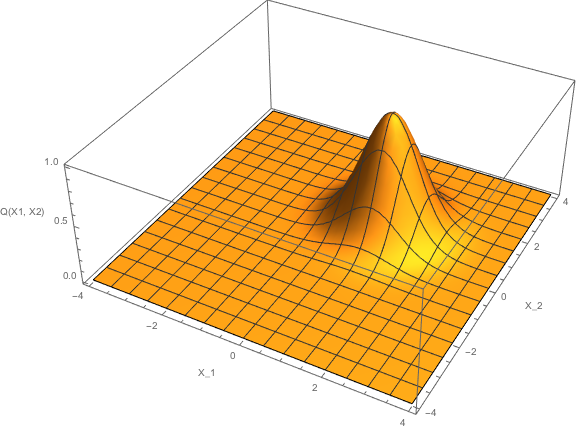
\includegraphics[width=\linewidth]{Q Function-Coherent.png}
	\end{minipage}%
  \begin{minipage}{0.5\linewidth}
          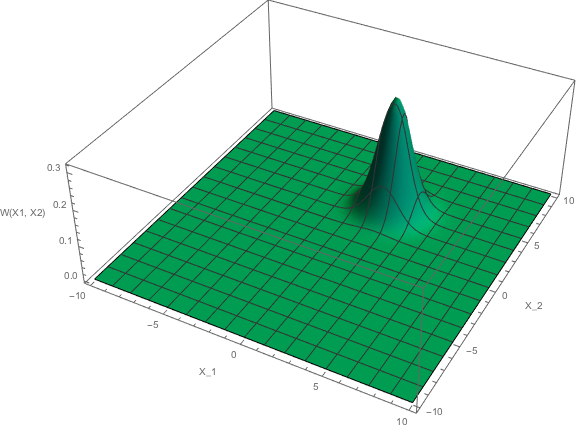
\includegraphics[width=\linewidth]{W Function-Coherent.png}
    \end{minipage}
  \caption{(a) Q function (orange) and Wigner Function (green) for the coherent states $\alpha = 1+i$ and $\alpha = 5+3i$}
\end{figure}
\subsection{Fock state representations}
\subsubsection{P-function}
Since Fock states have no classical analogue, we would expect the P function associated with the Fock state density matrix $\ket{n}\bra{n}$ should be highly singular or negative.
From \cite{Mehta1967}  P ($\alpha$) is non-singular (not more singular than a $\delta$-function) if and only if $ \bra{\beta} \dens \ket{\beta} e^{|\beta|^2} $ is square integrable.
But, using the Fock state expansion of the coherent states
\begin{align}
	 \bra{\beta} \dens \ket{\beta} e^{|\beta|^2}  &= e^{-|\beta|^2} \sum_{k=0}^\infty \frac {{\beta^*}^k}{k!} \braket{k}{n}\braket{n}{k} \sum_{k=0}^\infty \frac {\beta^k}{k!}e^{|\beta|^2} \\ &= e^{-|\beta|^2} \frac{|\beta|^{2n}}{{n!}^2} e^{|\beta|^2} \\ &= \frac{|\beta|^{2n}}{{n!}^2}
\end{align}
Which is square integrable for no value of n.

A representation in terms of a class of generalised functions called \emph{tempered distributions} is possible\footnote{Specifically, in terms of the derivatives of a Dirac delta function\cite{Gerry2005}}, but the behaviour of such objects makes them difficult to work with.
\subsubsection{Q-function}
Despite the pathological Fock state P-function the Q-function follows simply from the definition
\begin{align}
	 Q(\alpha) = \bra{\alpha} \dens \ket{\alpha}  &= \sum_{k=0}^\infty \frac {{\alpha^*}^k}{k!} \braket{k}{n}\braket{n}{k} \sum_{k=0}^\infty \frac {\alpha^k}{k!}e^{-|\alpha|^2} \\ &= \frac{|\alpha|^{2n}}{{n!}^2} e^{-|\alpha|^2}
\end{align}
\begin{figure}[ht]
	\begin{minipage}[b]{.5\linewidth}
        \centering \large 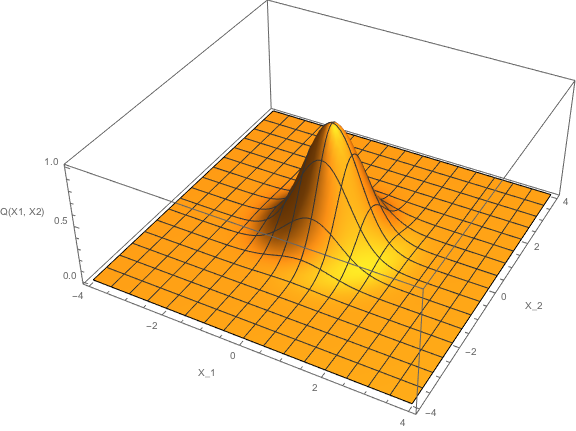
\includegraphics[width=1\linewidth]{Q Function-n=0.png}
	\end{minipage}%
	\begin{minipage}[b]{.5\linewidth}
		\centering\large 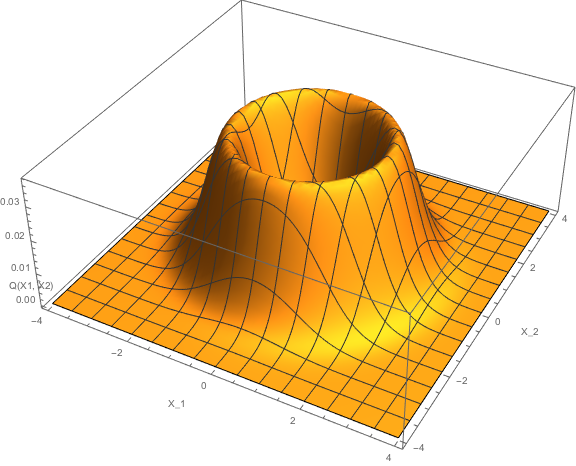
\includegraphics[width = 1\linewidth]{Q Function-n=3.png}
	\end{minipage}
  \caption{Fock State Q Functions for n=0 and n=5}\label{Qfunctions}
\end{figure}
\subsubsection{Wigner function}
The Wigner transform of $\ket{n}\bra{n}$ is\cite[65]{Walls2008}
\begin{equation}
	W(x_1, x_2) = \frac{2}{\pi} {(-1)}^n \mathscr{L}_n(4(x_1^2+x_2^2))e^{-2(x_1^2+x_2^2)}
\end{equation}
Where $\mathscr{L}_n$ is the nth Laguerre Polynomial.
\begin{figure}[ht]
	\begin{minipage}[b]{.5\linewidth}
		\centering \large 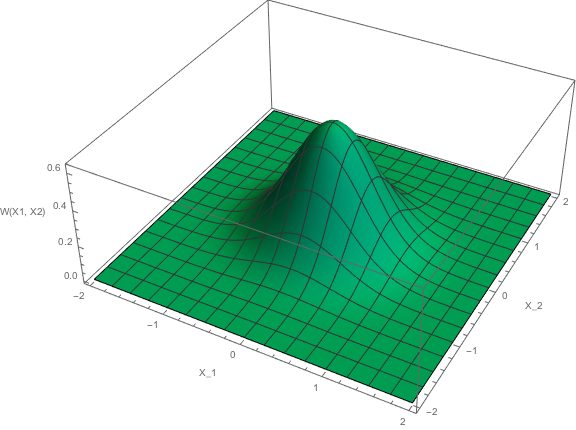
\includegraphics[width=1\linewidth]{W Function-n=0.png}
	\end{minipage}%
	\begin{minipage}[b]{.5\linewidth}
		\centering\large 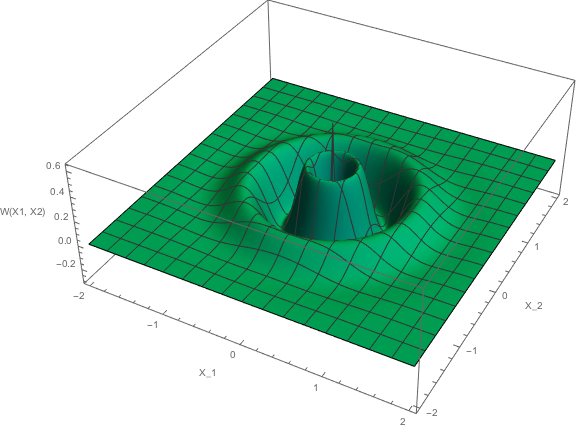
\includegraphics[width = 1\linewidth]{W Function-n=10.png}
	\end{minipage}
	\caption{Fock State Wigner Functions for n=0 and n=10}\label{Wfunctions}
\end{figure}
\subsection{Generalised P Representations}
Any density operator admits a diagonal P representation in terms of distributions, which are computationally and conceptually complicated.
The overcompleteness of the coherent states does not sufficiently restrict the P function, and thus they are not unique.
For this purpose the R representation was proposed \cite{Glauber1963a}. 
This representation does not generally yield positive definite Fokker-Planck diffusion matrices \cite{Walls2008}, and as such it has not seen much use.\\

Introducing an additional complex variable for a coherent basis {$\ket{\beta}_{\beta\in\mathbb{C}}$}, a measure $d\mu(\alpha, \beta)$ and an integration domain $\mathscr{D}\subset\mathbb{C}\times\mathbb{C}$ defines a family of representations of the density matrix, which have had substantial analytical success
\cite{Drummond1979}.
This formalism is due to \cite{Drummond1980}.
The extension goes 
\begin{equation}
  \dens = \iint_{\alpha, \beta \in \mathscr{D}}P \left( \alpha, \beta \right) \hat{\mathscr{J}} 
          d \mu \left( \alpha, \beta \right)
\end{equation}
with
\begin{equation}
  \hat{\mathscr{J}} = \frac{\ket{\alpha}\bra{\beta^*}}{\braket{\beta^*}{\alpha}} 
\end{equation}
We trade a real (quasi-)probability function over a real (classical) phase space, for a (generally) complex function of two complex variables, on a complex phase space.
\subsubsection{Diagonal} 
The measure that recovers the diagonal P representation is
\begin{equation}
  d\mu(\alpha, \beta) = \delta(\alpha-\beta^*)d^2 \alpha d^2 \beta
\end{equation}
$\alpha$ and $\beta = \alpha^*$ now take values on a two-dimensional subset of the complex plane ($\mathbb{C}\times\mathbb{C}$) - the familiar real phase plane.
\subsubsection{Complex}
Letting $\beta, \alpha$ vary independently on two different complex contours $\mathscr{C}, \mathscr{C}'$, and taking as measure
\begin{equation}
  d\mu\left(\alpha, \beta\right) = d\alpha d\beta
\end{equation}
The corresponding P function can take complex values.
This representation has been used to derive the photon number distribution of a cavity containing a nonlinear medium \cite{Drummond1979}.
\subsubsection{Positive}
We consider a surface integral over the whole $\alpha$-$\beta$ plane
\begin{equation}
  d \mu(\alpha, \beta) = d^2 \alpha d^2 \beta
\end{equation}
In this case the distribution is always positive, and always admits an interpretation as a genuine probability. 
\subsection{Stochastic Processes \& Fokker-Planck Equations}
Here we talk about stochastic processes and Fokker-Planck equations in quantum optics 
\cite{Carmichael1992} 
\cite{Carmichael2008} 
\cite{Breuer2002} 
\subsection{Application}
Here we consider a cavity containing a nonlinear medium, driven by a coherent field. \cite{Drummond1979}
\section{Circuit QED}
Circuit QED (cQED) is a promising paradigm for the implementation of quantum computation, as well as in quantum information and simulation.
The DiVincenzo Criteria \cite{DiVincenzo} provide a set of requirements for a scalable quantum computer. 
Of them, the most important in cQED is decoherence. 
\subsection{cQED qubits}
There are several scalable well-characterised qubit candidates in superconducting circuits\cite{Makhlin2001}.
They fall into distinct types based on the quantum degree of freedom they exploit: phase, charge, or flux.
Here we look at a particular type of charge qubit: the \emph{transmon}.
\subsection{Cooper Pair Box}
The transmon is an improvement on the Cooper Pair Box(CPB) qubit.
In the CPB, a superconducting island is coupled through a Josephson junction and a capacitance to a voltage.
\begin{figure}[t]
  \includegraphics[width=\linewidth]{cpb.png}
  \caption{Schematic of a Cooper Pair Box. Island is demarcated by the dashed line.}
\end{figure}
The system is described by the Hamiltonian\cite{Makhlin2001}
\begin{equation}
  \mathscr{H} = 4E_C(n-n_g)^2 - E_J \cos \Theta
\end{equation}
where n is the number of excess cooper pairs on the island, $\Theta$ the (conjugate) phase of the island superconducting order parameter, $E_J$ is the Josephson energy, $E_C$ the charging energy, and $n_g$ the dimensionless gate charge.
We can represent this hamiltonian in the charge basis:
\begin{align}
  \mathscr{H} &= \sum_n \Bigg\{ 4 E_C (n-n_g) \ketbra{n}{n}\\ 
              &- \frac{1}{2} E_J \left( \ketbra{n}{n+1} 
                                       + \ketbra{n+1}{n} \right) \Bigg\}
\end{align}
tuning $n_g$, we can select strongly just two states, and cast this hamiltonian into 2 level form.
\begin{equation}
  \mathscr{H} = 2E_C ( 1-2n_g ) \sigma_z - E_J \sigma_x 
\end{equation}
\subsection{Transmon}
There are two conflicting goals for an effective qubit. 
There must be a highly anharmonic level system, where one transition can be strongly addressed in isolation. 
Noise must be suppressed so that the qubit state can be faithfully read out and controlled. 
In the Cooper Pair Box, these goals are orthogonal.
\begin{figure}[t]
  \includegraphics[width=\linewidth]{anharmonicity.png}
  \caption{CPB level scheme as a function of the dimensionless gate charge $n_g$ \cite{Koch2007}}
  \label{anharmonicity}
\end{figure}
In \ref{anharmonicity} this behaviour is obvious. 
For low $\frac{E_J}{E_C}$, The greatest level anharmonicity is achieved by operating the qubit at the half integer charge degeneracy points.
At this point the gradient is zero and first order fluctuations are suppressed. 
However, the change in the transition width with small changes in gate charge is great. 
In contrast, for high $\frac{E_J}{E_C}$ this noise sensitivity disappears, at the cost of a great deal of level anharmonicity.
The transmon exploits the fact that the decrease of charge noise with increasing $\frac{E_J}{E_C}$ is exponential, while the decrease in anharmonicity is algebraic.
The transmon is a cooper pair box with an additional shunting capacitance $C_B$, and an additional parallel Josephson junction.
\begin{figure}[t]
  \includegraphics[width=\linewidth]{transmon.png}
  \caption{Schematic of a transmon. Island is highlighted in dark blue\cite{Koch2007}.}
\end{figure}
The shunting capacitance changes the noise behaviour of the device significantly.
While the transmon hamiltonian takes the same form as the CPB system, the additional capacitance suppresses the charging energy $E_C$ relative to the CPB.
This changed charging energy suppresses system noise at the cost of only a small amount of anharmonicity. 

We take these qualities as those of a qubit, and couple the two level transmon system to a single electromagnetic field mode.
This is the Jaynes-Cummings system of Quantum Optics.
\section{The Jayes-Cumming Hamiltonian}
In the Jaynes-Cummings model, a single cavity mode interacts with a two level system. 

We start with the total Hamiltonian
\begin{equation}
	\mathscr{H} = \mathscr{H}_A + \mathscr{H}_F +\mathscr{V}_{int}
\end{equation}
\subsection{The Dipole Approximation}
In full generality, the field will interact with all the higher order dipole moments of the atom.
However, given that the spatial variation of typical optical fields is minimal on the order of an atom ($\sim$ \AA), the interaction hamiltonian can be approximated by the interaction of the electric field only with the electric dipole moment of the atom
\begin{equation}
	\hat{\mathscr{V}}_{int} = -\vec{\hat{d}} \cdot \vec{\hat{E}}
\end{equation}
The quantized electromagnetic multimode vector potential in a medium can be expressed in the following way \cite[271--273]{Novotny2006}(we consider only a countable number of field modes, since we will put the field in a cavity)
\begin{equation}
	\hat{A} = \sum_{\vec{k}, \mu} \sqrt{\frac{\hbar}{2\omega_{\vec{k}} V \varepsilon_0}} (\vec{u}_{\vec{k}} \ann + \vec{u}^*_{\vec{k}} \cre )
\end{equation}
with $\vec{u}_{\vec{k}}$ orthogonal normal modes satisfying the wave equation:
\begin{equation}
	\nabla \times \nabla \times \vec{u}_{\vec{k}} = \frac{\omega_{\vec{k}}^2}{c^2}  \vec{u}_{\vec{k}}
\end{equation}
We consider only coupling to a single mode of the cavity field:
\begin{equation}
	\hat{A} =  \sqrt{\frac{\hbar}{2\omega_{\vec{k}} V \varepsilon_0}} (\vec{u}_{\vec{k}} \ann + \vec{u}^*_{\vec{k}} \cre )
\end{equation}
from which $\vec{E}$ for the mode is easily derived since (in the radiation gauge)
\begin{equation}
	\vec{\hat{E}} = -\frac{\partial}{\partial t}\vec{\hat{A}}
\end{equation}
\subsection{Two Level Approximation}
$\vec{\hat{d}} = e \vec{\hat{r}}$ can be expanded in the space of atomic levels by resolving unity on each side
\begin{equation}
	\vec{\hat{d}} = e \sum_{a, b} | a \rangle \langle a | \vec{\hat{r} }| b \rangle \langle b |
\end{equation}
since we consider only two levels, the sum can be truncated:
\begin{equation}
	\vec{\hat{d}} = e\{| 1 \rangle \langle 1|\vec{\hat{r}} | 1 \rangle \langle 1 | + | 1 \rangle \langle 1|\vec{\hat{r}} | 2 \rangle \langle 2 | + | 2 \rangle \langle 2|\vec{\hat{r}} | 1 \rangle \langle 1 | + | 2 \rangle \langle 2|\vec{\hat{r}} | 2 \rangle \langle 2 | \}
\end{equation}
we assume the atom has no permanent dipole moment and neglect terms of the form $| 1 \rangle \langle 1|\vec{\hat{r}} | 1 \rangle \langle 1 |$.
Expressing in terms of the atomic creation and annihilation operators
\begin{equation}
	\vec{\hat{d}} = (m\sigma_+ + m^* \sigma_-)
\end{equation}
where $m, m^*$ are the electric dipole matrix elements
\subsection{The Rotating Wave Approximation}
The free field hamiltonian, neglecting the zero point energy has the form
\begin{equation}
	\ham_F =  \hbar \omega \cre \ann
\end{equation}
The atom energy, neglecting centre of mass motion and considering only population inversion, in terms of the Pauli z matrix:
\begin{equation}
	\ham = \frac {1} {2} \hbar \omega_A \sigma_z
\end{equation}
where $\omega_A$ is the frequency of the bare atomic transition
Assuming sinusoidal mode functions with polarisation $\varepsilon_\Omega$, and incorporating constants into new dipole matrix elements $g = \frac{m \varepsilon_\Omega sin(Kz)} {2 \hbar}$, the total hamiltonian takes the form
\begin{equation}
	\ham = \hbar \omega \cre \hat{a} +\frac{1}{2} \hbar \omega_A \sigma_Z + \hbar (\ann +\cre)(g\atann+g^*\atcre)
\end{equation}
expanding the interaction term
\begin{equation}
	\hat{\mathscr{V}}_{int} = \hbar (\ann +\cre)(g\atann+g^*\atcre) =  \hbar (g \ann \atann + g^* \ann \atcre + g \cre \atcre +g^* \cre\atann)
\end{equation}
moving to an interaction picture rotating at the transition frequency $\omega_A$ it can be seen that terms of the form $\atann \cre $ counterrotate with frequency $\omega + \omega_L$ and terms of the form $ \atann \ann$ co rotate with frequency given by the detuning $\omega-\omega_L$.
The rotating wave approximation is the assumption that the counterrotating terms will quickly average to zero on the system timescale, and thus can be dropped in the expansion of the interaction hamiltonian.
\subsection{The Jaynes-Cumming Hamiltonian}
Applying all of the above leads to a hamiltonian $\ham_{JC}$ of the form:
\begin{equation}
	\ham_{JC} = \hbar \omega \cre \hat{a} +\frac{1}{2} \hat{\sigma}_Z \omega_A + \hbar g (\cre \atann + \hat{a} \atcre)
\end{equation}
\subsection{Solving the Jaynes Cumming system in the absence of drive}
We first move to an interaction picture rotating with the bare system, partitioning the Hamiltonian
\begin{align}
	\ham_I &= \hbar \omega \hat{N}_e + \hbar(\frac{\omega_A}{2}-\omega)\hat{P}_E \\
	\ham_{II} &= -\hbar \Delta + \hbar g (\cre \atann + \hat{a} \atcre) \\
	\ham_{JC} &= \ham_I+\ham_{II}
\end{align}
with $\Delta = \omega-\omega_A$,   $\hat{N}_e = \ket{2} \bra{2} + \ket{1} \bra{2} $ the (conserved) electron number and $\hat{P}_E = \cre\ann + \ket{2}\bra{2} $ the (conserved) excitation number.
We allow the kets and observables to evolve with the conserved part, and solve for the interesting dynamics in the interaction part.
\subsection{Unitary, zero detuning}
We consider first evolution of the Jaynes-Cumming system in the absence of decay, dephasing and detuning.
Since the field only couples successive levels of the combined atom-field system, the state of the closed system can be described in the restricted two level Hilbert space
\begin{equation}
	\ket{\psi(t)} = C_1(t) \kettens{1}{g} + C_2(t) \kettens{0}{e}
\end{equation}
where $\ket{\psi}$ is understood to be an element of the atom-field Hilbert space.
We solve the interaction schrodinger equation to determine the time dependent coefficients $C_1(t)$ and $C_2(t)$
\begin{equation}
	\schro{\psi(t)}{\ham_{II}}
\end{equation}
and get two coupled differential equations for the level amplitudes:
\begin{align}
	\frac{d C_2(t)}{dt} &= -i g \sqrt{n+1}C_1(t)\\
	\frac{d C_1(t)}{dt} &= -i g \sqrt{n+1}C_2(t)
\end{align}
\subsubsection{Solutions}
Here we plot the sin and cos solutions to the above. 
\subsection{Initial Conditions}
\subsubsection{Fock State}
\subsubsection{Coherent State}
\subsubsection{Rabi Flopping}
\subsection{Solving the Jaynes Cummings system in the presence of drive}
Here we desribe the canonical transformation that we later use.
We discuss coherent and incoherent driving.
